\documentclass[a4paper,10pt,fleqn]{article}
\usepackage{tex/00/layout}

\usepackage{float}		% Allow floating pictures
\usepackage{url}
\usepackage{todonotes}    %Todo notes
\usepackage{pdfpages}	% Insert pdf in documentation

\tolerance=500            % hbox badness warning supression

%%%%%%%%%%%%%%%%%%%%%%%%%%%%%%%%%%%%%%%%%%%%%%%%%%%%%%%%%%%
\begin{document}


% Title

\begin{titlepage}
	\centering
	
\includegraphics[width=0.15\textwidth]{pic/00_title/logo.png}
	\par\vspace{1cm}
	{\scshape\LARGE Hochschule Luzern - Technik \& Architektur \par}
	\vspace{1cm}
	{\scshape\Large EAT - Labor\par}
	\vspace{1.5cm}
	{\huge\bfseries Wechselrichter einphasig\par}
	\vspace{2cm}
	%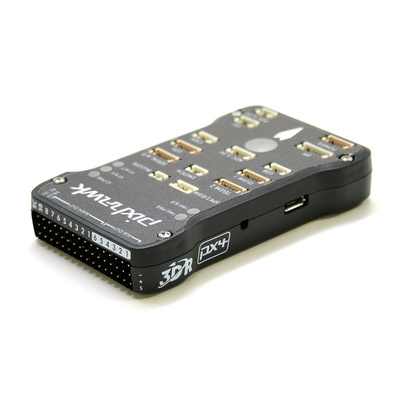
\includegraphics[width=0.35\textwidth]{pic/00_title/title.jpg}
	%\par\vspace{1cm}
	{\Large\itshape Pascal Häfliger\par}
	{\Large\itshape Cyrill Knüsel\par}
	\vfill
	betreut durch:\par
	Prof.~Dr.~ Adrian \textsc{Omlin}\par
	\vspace{1cm}
	

	\vfill  % Rest der Titelseite mit Leerraum auffüllen

% Bottom of the page
	{\large \today\par}
\end{titlepage}



\clearpage
% Inhaltsverzeichniss
\tableofcontents
\clearpage



% Messungen
\section{Messungen}

\noindent Schema:

\begin{figure}[H]
  \begin{center}
  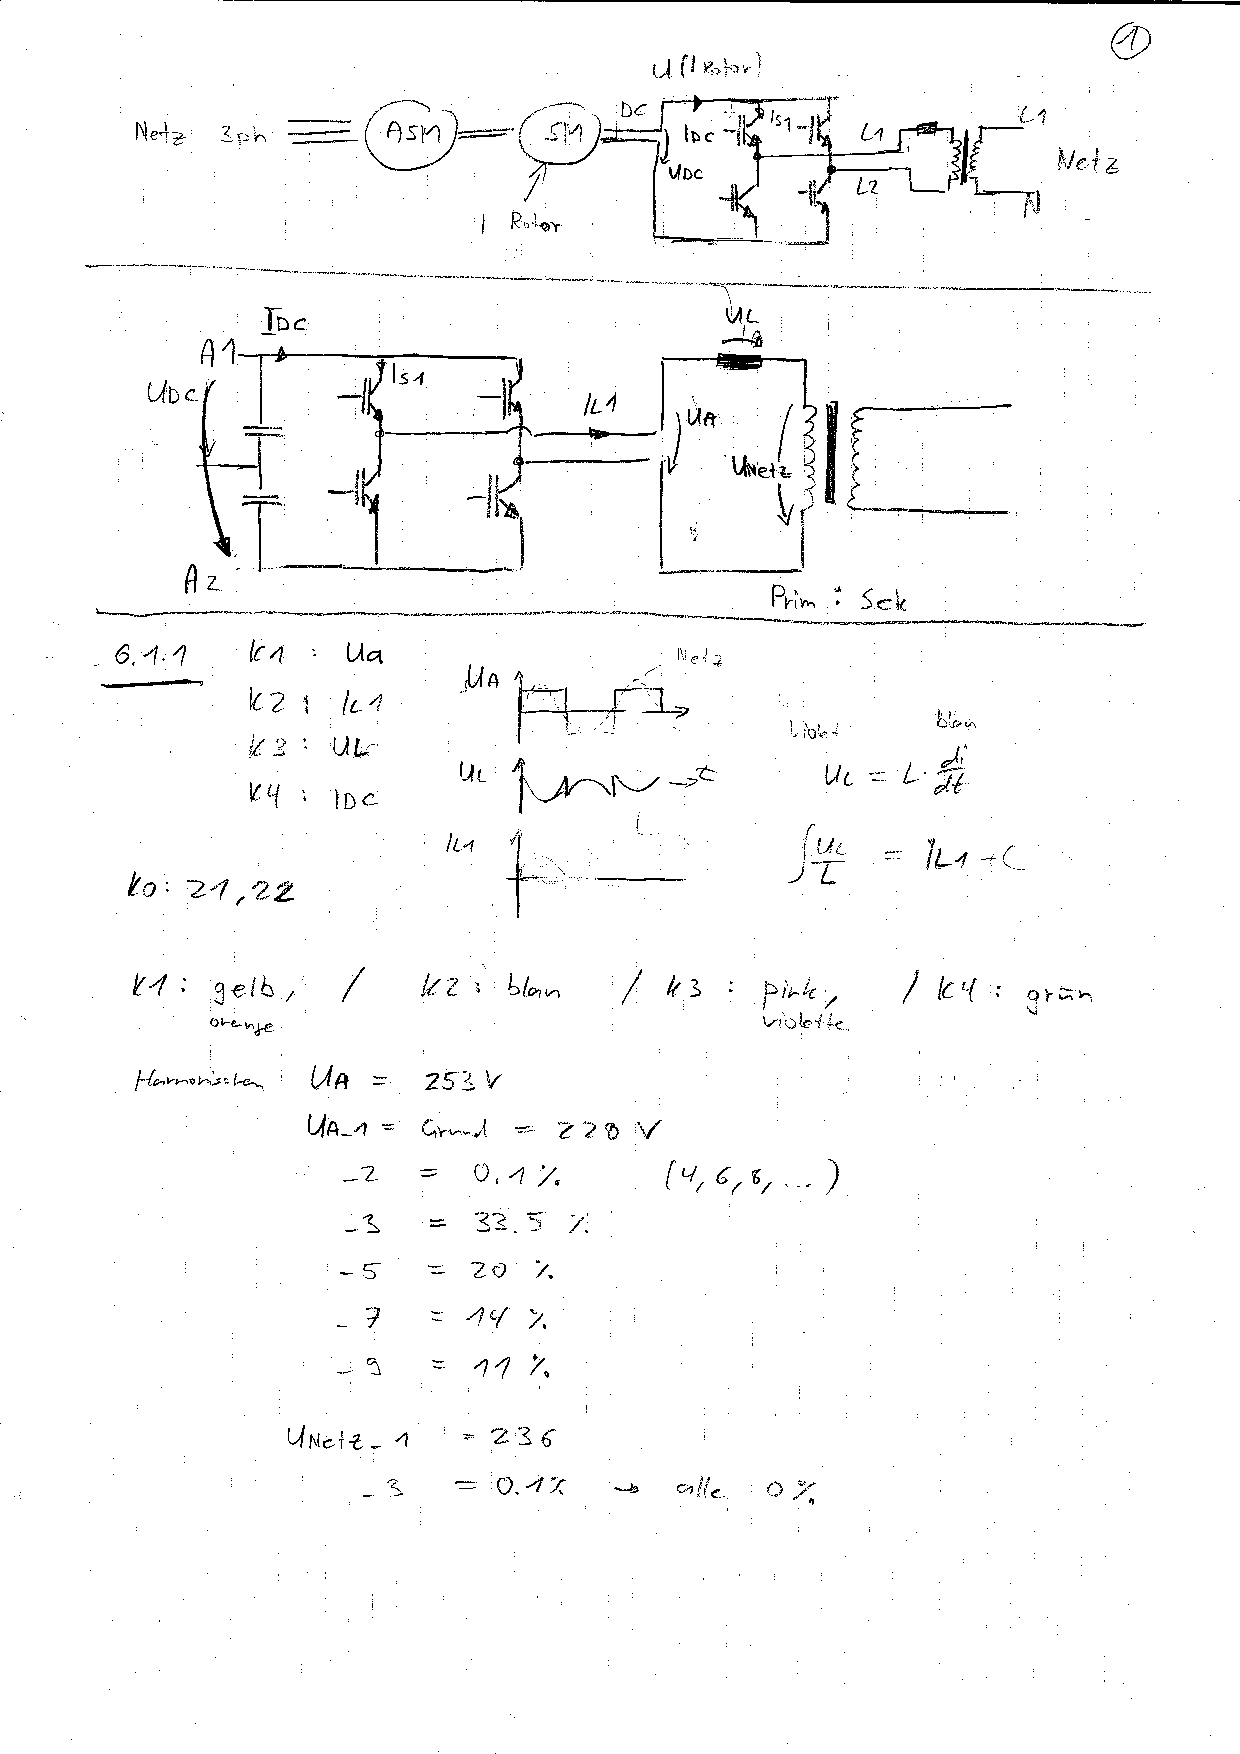
\includegraphics[width=1\textwidth, trim={1cm 19.38cm 1cm 5cm},clip]{notes/scan1.pdf}
  \caption{Schema}
  \label{fig:schema}
  \end{center}
\end{figure}


Kanalbelegung beim KO:


\begin{table}[h]
  \centering
  \begin{tabular}{ l | l | l }
    \hline 
    Channel & Farbe & Bezeichnung \\
    \hline \hline
    1 & gelb / orange &  $U_A$ \\
    \hline
    2 & hellblau & $I_{L1}$ , da Einphasig\\  
    \hline 
    3 & pink / violette & $U_{L}$ \\  
    \hline
    4 & grün & $I_{DC}$ \\  
    \hline
  \end{tabular}
  \caption{Kanalbelegung}
  \label{tab:Kanalbelegung}
\end{table}




\clearpage

\subsection{Grundfrequenztaktung}



\clearpage
\subsubsection{Stromform}
Folgende Einstellungen wurden bei diesem Versuch vorgenommen:
\begin{itemize}
\item Winkel $\alpha = 0°$
\item Wechselrichter ist mit dem Netz synchronisiert.
\end{itemize}

Die Spannung $U_L$ ist die zeitliche Ableitung des Stromes multipliziert mit der Induktivität.
\begin{center}
$U_L = L * \frac{di}{dt}$
\end{center}

\begin{figure}[H]
  \begin{center}
  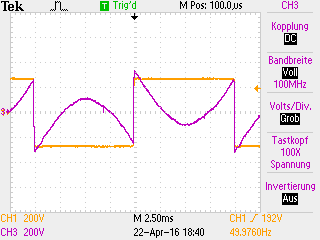
\includegraphics[width=0.48\textwidth]
  {pic/6_1_grundfrequenztaktung/6_1_1_stromform/ALL0001/F0001TEK.png}
  \caption{$U_A$ (orange) , $U_L$ (violett)}
  \label{fig:6_1_1_1}
  \end{center}
\end{figure}


Die Strom $I_L$ ist das Integral der Spannung $U_L$ geteilt durch die Induktivität, zuzüglich des Startwerts.
\begin{center}
$I_L = \frac{1}{L} * \int U_L dt$
\end{center}
\begin{figure}[H]
  \begin{center}
  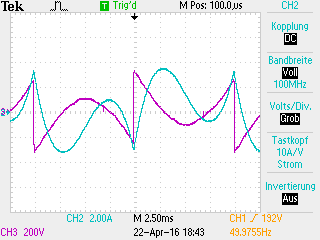
\includegraphics[width=0.48\textwidth]
  {pic/6_1_grundfrequenztaktung/6_1_1_stromform/ALL0002/F0002TEK.png}
  \caption{$U_L$ (violett), $I_{L1}$ (blau)}
  \label{fig:6_1_1_2}
  \end{center}
\end{figure}

Nur die Wechselrichterspannung $U_A$ enthält harmonische Oberschwingungen, nämlich alle ungeraden. Anhand der Tabelle \ref{tab:harm_wr} sieht man, dass die Amplitude der v-ten Oberschwingung jeweils um $1/v$ kleiner ist als die der Grundschwingung.

\begin{table}[h]
  \centering
  \begin{tabular}{ l | l | l }
    \hline 
    Harmonische  & Wert & Einheit \\
    \hline \hline
    $U_A$ eff. & 253  &  V\\
    \hline
    $U_A$ 01   & 220  &  V\\  
    \hline 
    $U_A$ 02   & 0.1  &  \%\\  
    \hline
    $U_A$ 03   & 33.5 &  \%\\  
    \hline
    $U_A$ 05   & 20   &  \%\\  
    \hline
    $U_A$ 07   & 14   &  \%\\  
    \hline
    $U_A$ 09   & 11   &  \%\\  
    \hline
  \end{tabular}
  \caption{Harmonische der Wechselrichterspannung $U_A$}
  \label{tab:harm_wr}
\end{table}

\begin{table}[h]
  \centering
  \begin{tabular}{ l | l | l }
    \hline 
    Harmonische  & Wert & Einheit \\
    \hline \hline
    $U_A$ 01   & 220  &  V\\  
    \hline 
    $U_A$ 03   & 0.1  &  \%\\  
    \hline
  \end{tabular}
  \caption{Harmonische der Netzspannung}
  \label{tab:harm_netz}
\end{table}



\clearpage
\subsubsection{Einstellen von Wirk- und Blindleistung}
Bei dieser Messung wurde die Wirk- bzw. Blindleistung anhand des Zündwinkels und der DC-Spannung (Zündwinkel $\theta = 0°$) eingestellt. \\

Für den Effektivwert wurde die Wirk- bzw. Blindleistung folgendermassen ausgerechnet. \\
$S = U*I, U=const$
P abgelesen
$Q = \sqrt{(S^2 - P^2)}$
\begin{figure}[!ht]
  \begin{center}
  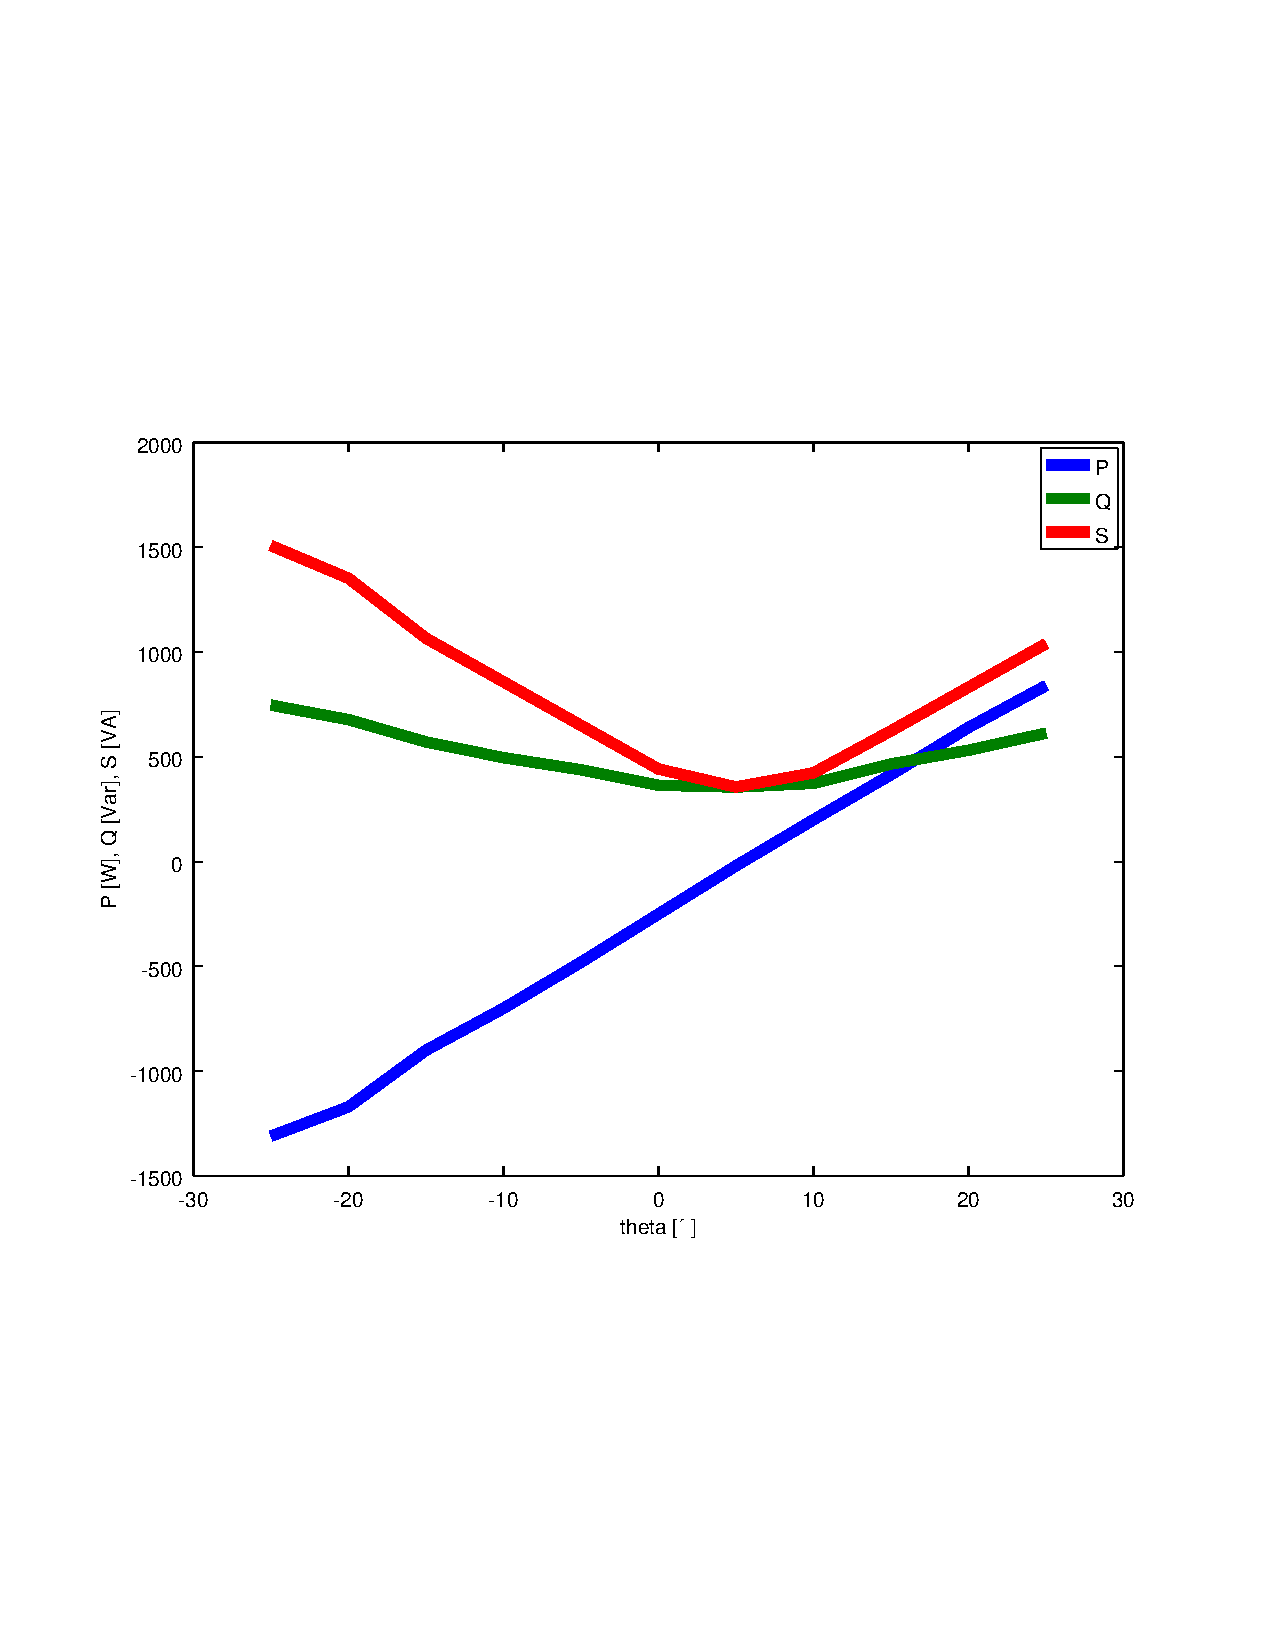
\includegraphics[width=0.5\textwidth, trim={1cm 6.5cm 2cm 7cm},clip]{pic/6_1_grundfrequenztaktung/6_1_2_einst_wirk_und_blindleistung/P_Q_S.pdf}
  \caption{$P(\theta) (blau), Q(\theta) (grün), S(\theta) (rot)$ von dem Effektivwert in Abhängigkeit des Zündwinkels}
  \label{fig:6_1_2_0}
  \end{center}
\end{figure}


Für die Grundschwingung wurde die Wirk- bzw. Blindleistung folgendermassen ausgerechnet.\\
$S_1 = U_1 * I_1$
\underline{I1} abgelesen, Trigger auf Strom
$P_1 = S_1 * cos(\phi)$
$Q_1 = S_1 * sin(\phi)$
\begin{figure}[!ht]
  \begin{center}
  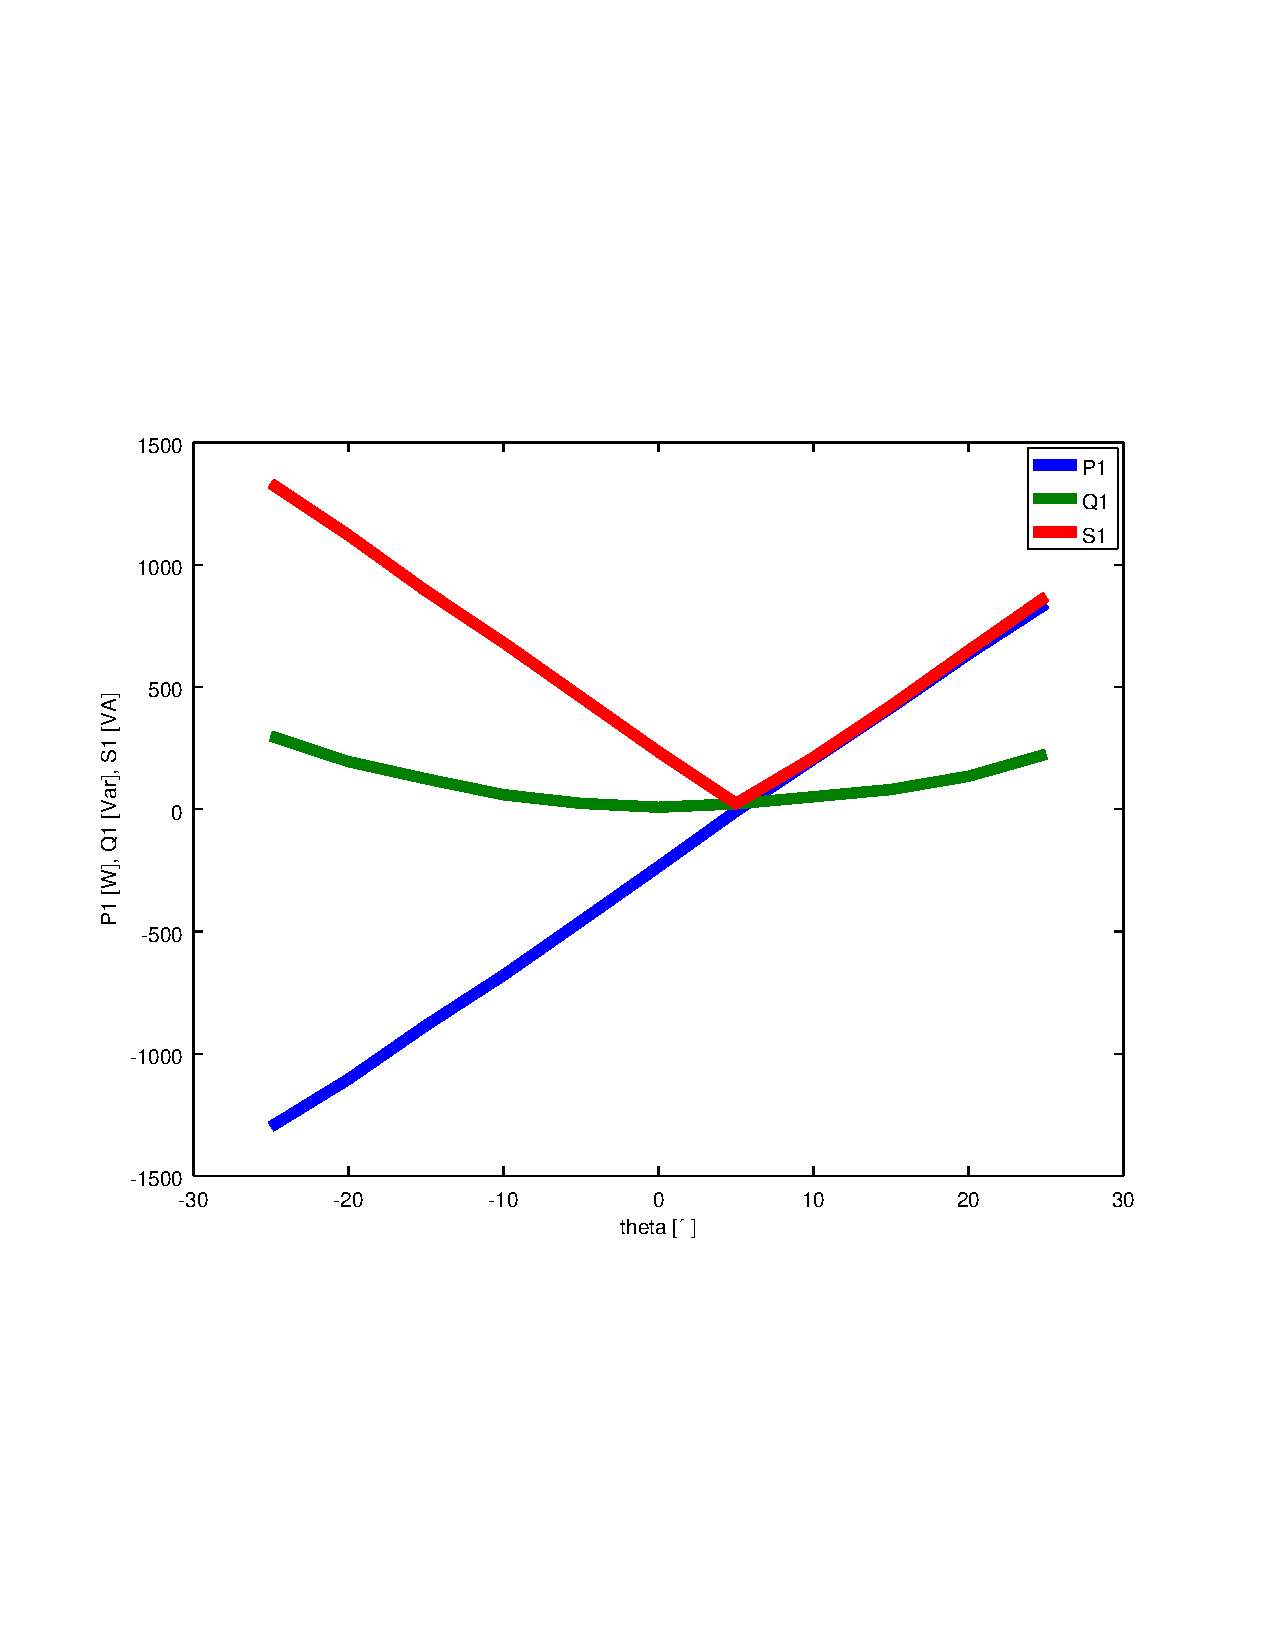
\includegraphics[width=0.5\textwidth, trim={1cm 6.5cm 2cm 7cm},clip]{pic/6_1_grundfrequenztaktung/6_1_2_einst_wirk_und_blindleistung/P1_Q1_S1.pdf}
  \caption{$P1(\theta) (blau), Q1(\theta) (grün), S1(\theta) (rot)$ von dem Effektivwert in Abhängigkeit des Zündwinkels}
  \label{fig:6_1_2_1}
  \end{center}
\end{figure}

Die folgenden zwei Abbildungen zeigen nochmals die Wirk- bzw. Blindleistung im direkten Vergleich.


\begin{figure}[H]
  \begin{center}
  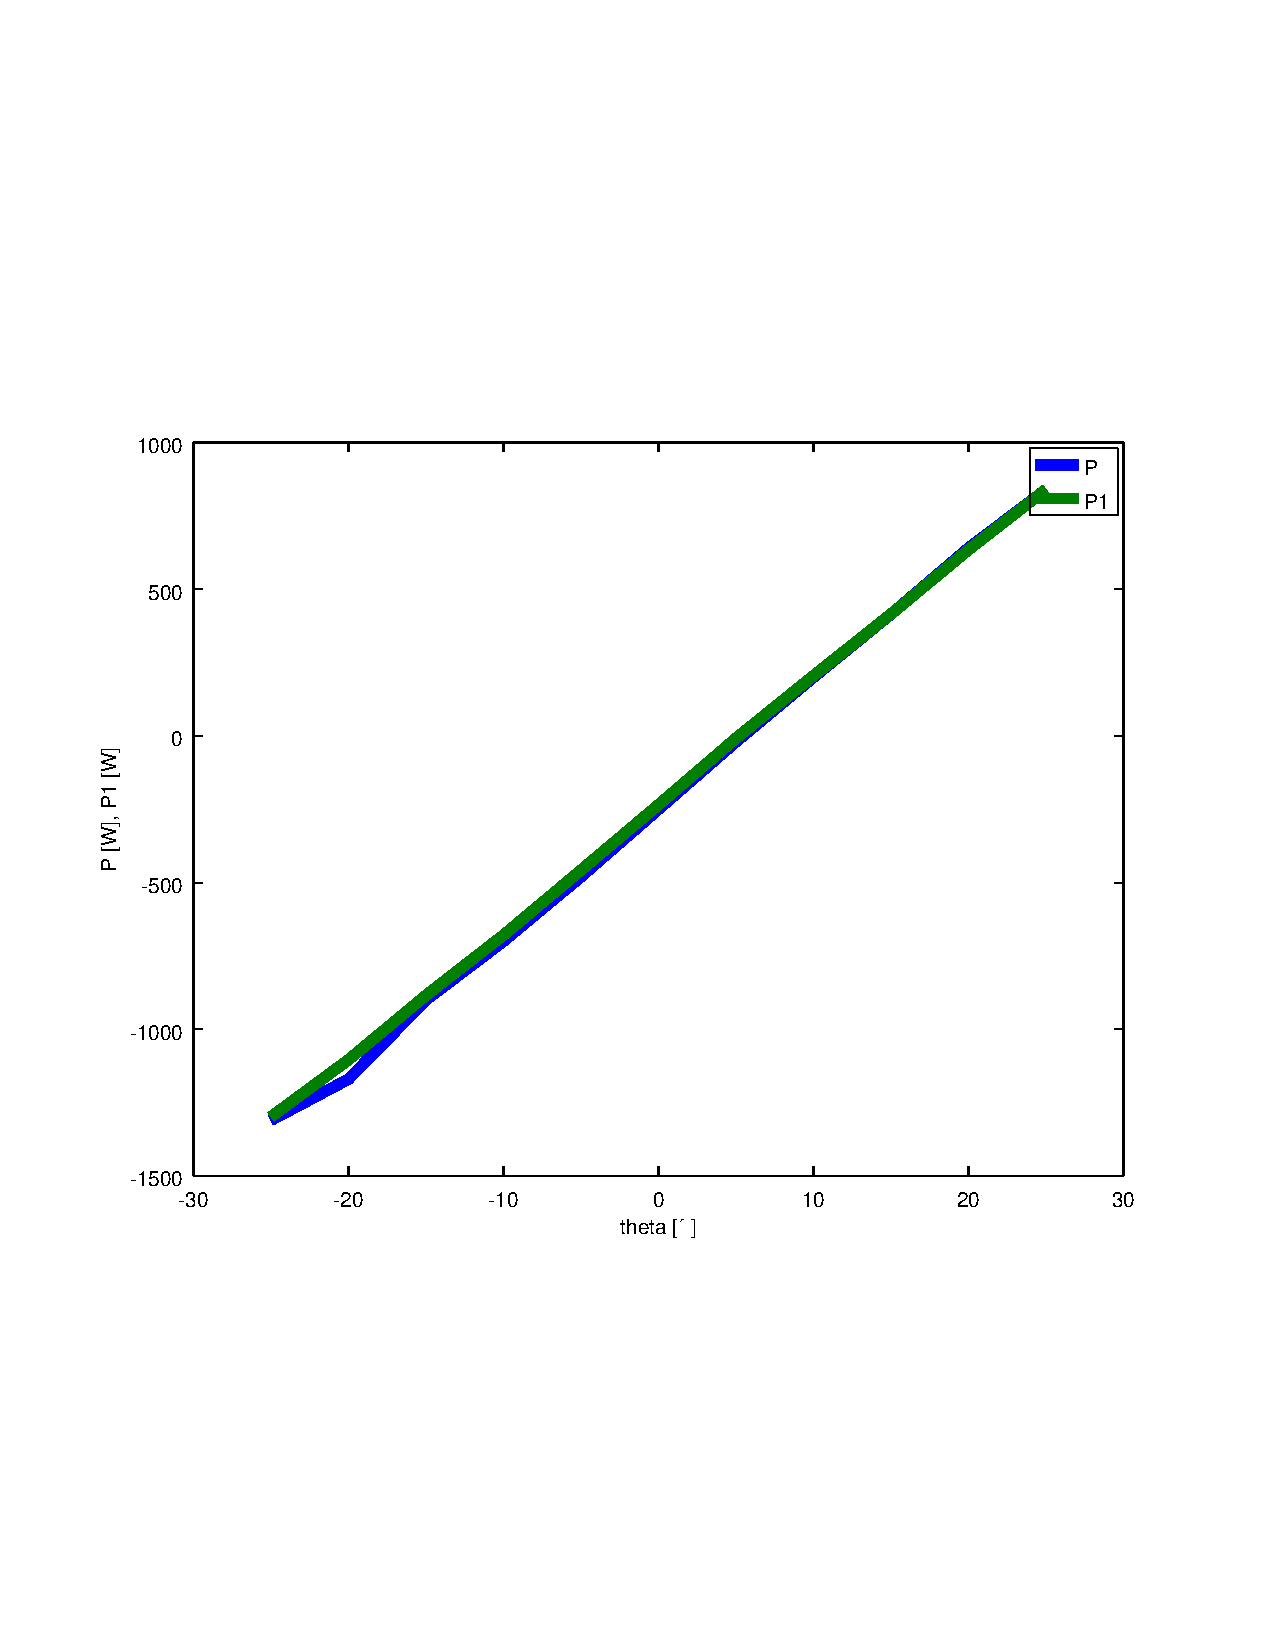
\includegraphics[width=0.5\textwidth, trim={1cm 6.5cm 2cm 7cm},clip]{pic/6_1_grundfrequenztaktung/6_1_2_einst_wirk_und_blindleistung/P_P1.pdf}
  \caption{Wirkleistung $P(\theta)(blau), P1(\theta) (grün)$ in Abhängigkeit des Zündwinkels}
  \label{fig:6_1_2_2}
  \end{center}
\end{figure}

Auffallend ist, dass beim Zündwinkel von $-30°$ die gesamte Wirkleistung kleiner ist als die der Grundschwingung. Eine mögliche Begründung wäre, dass in diesem Betriebspunkt die harmonischen Oberschwingungen zusätzlich Wirkleistung erzeugen und dies das Leistungsmessgerät beim Effektivwert nicht berücksichtigt.


\begin{figure}[H]
  \begin{center}
  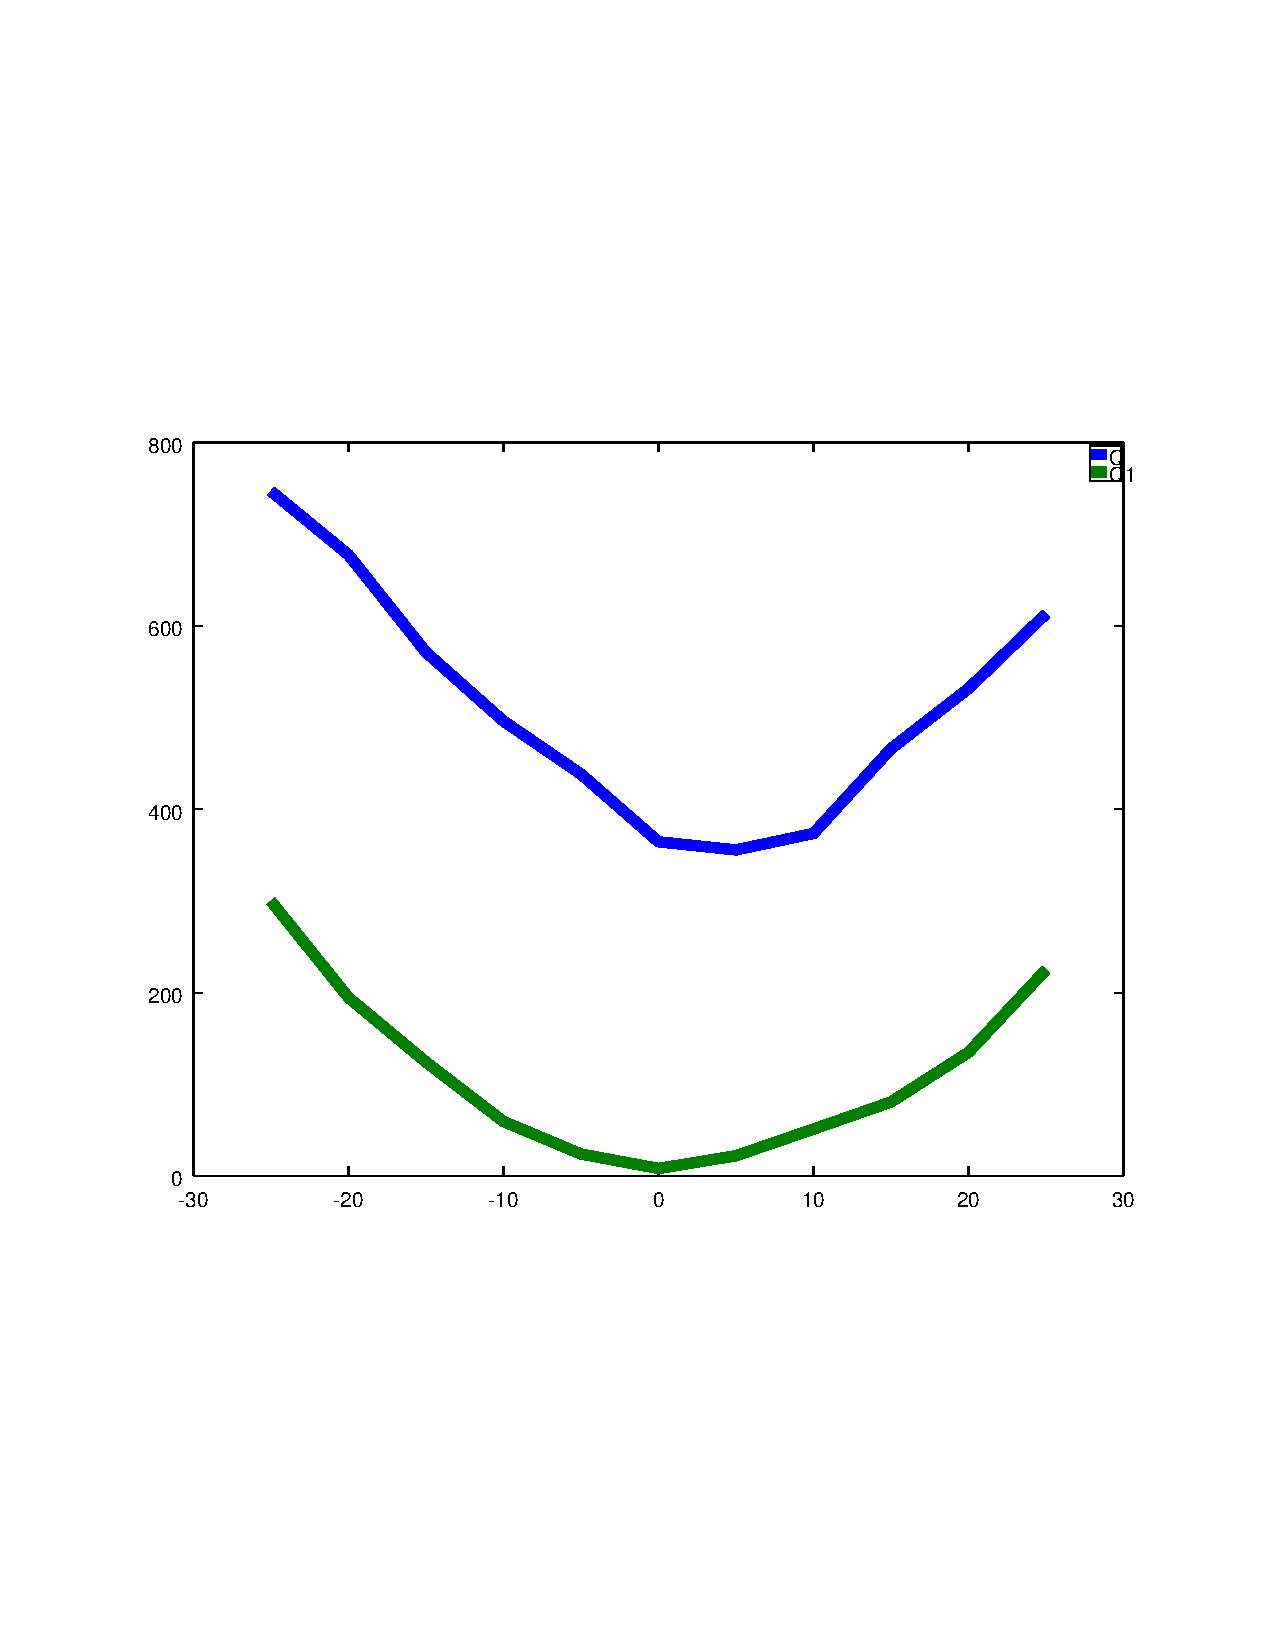
\includegraphics[width=0.5\textwidth, trim={1cm 6.5cm 2cm 7cm},clip]{pic/6_1_grundfrequenztaktung/6_1_2_einst_wirk_und_blindleistung/Q_Q1.pdf}
  \caption{Blindleistung $Q(\theta) (blau), Q1(\theta) (grün)$ in Abhängigkeit des Zündwinkels}
  \label{fig:6_1_2_3}
  \end{center}
\end{figure}
Die Blindleistung ist immer positiv da diese mit hilfe des Quadrats berechnet wurde.\\
Anhand der Abbildungen \ref{fig:6_1_2_0} - \ref{fig:6_1_2_3} ist zu sehen, dass der eingestellte Zündwinkel von $\theta = 5°$ dem effektiven Winkel von $0°$ entspricht. Denn in diesem Punkt gibt der Wechselrichter weder Wirkleistung ab noch bezieht er Wirkleistung.\\

Die Abbildungen \ref{fig:6_1_2_4} und \ref{fig:6_1_2_5} zeigen die Wirk- bzw. Blindleistung in Abhängigkeit von der Gleichspannung. Bei 310 Volt war der Wechselrichter synchron und der eingestellte Zündwinkel betrug $0°$.\\

$S = U * I$
I und P abgelesen
$Q = sqrt{S^2 - P^2}$

\begin{figure}[H]
  \begin{center}
  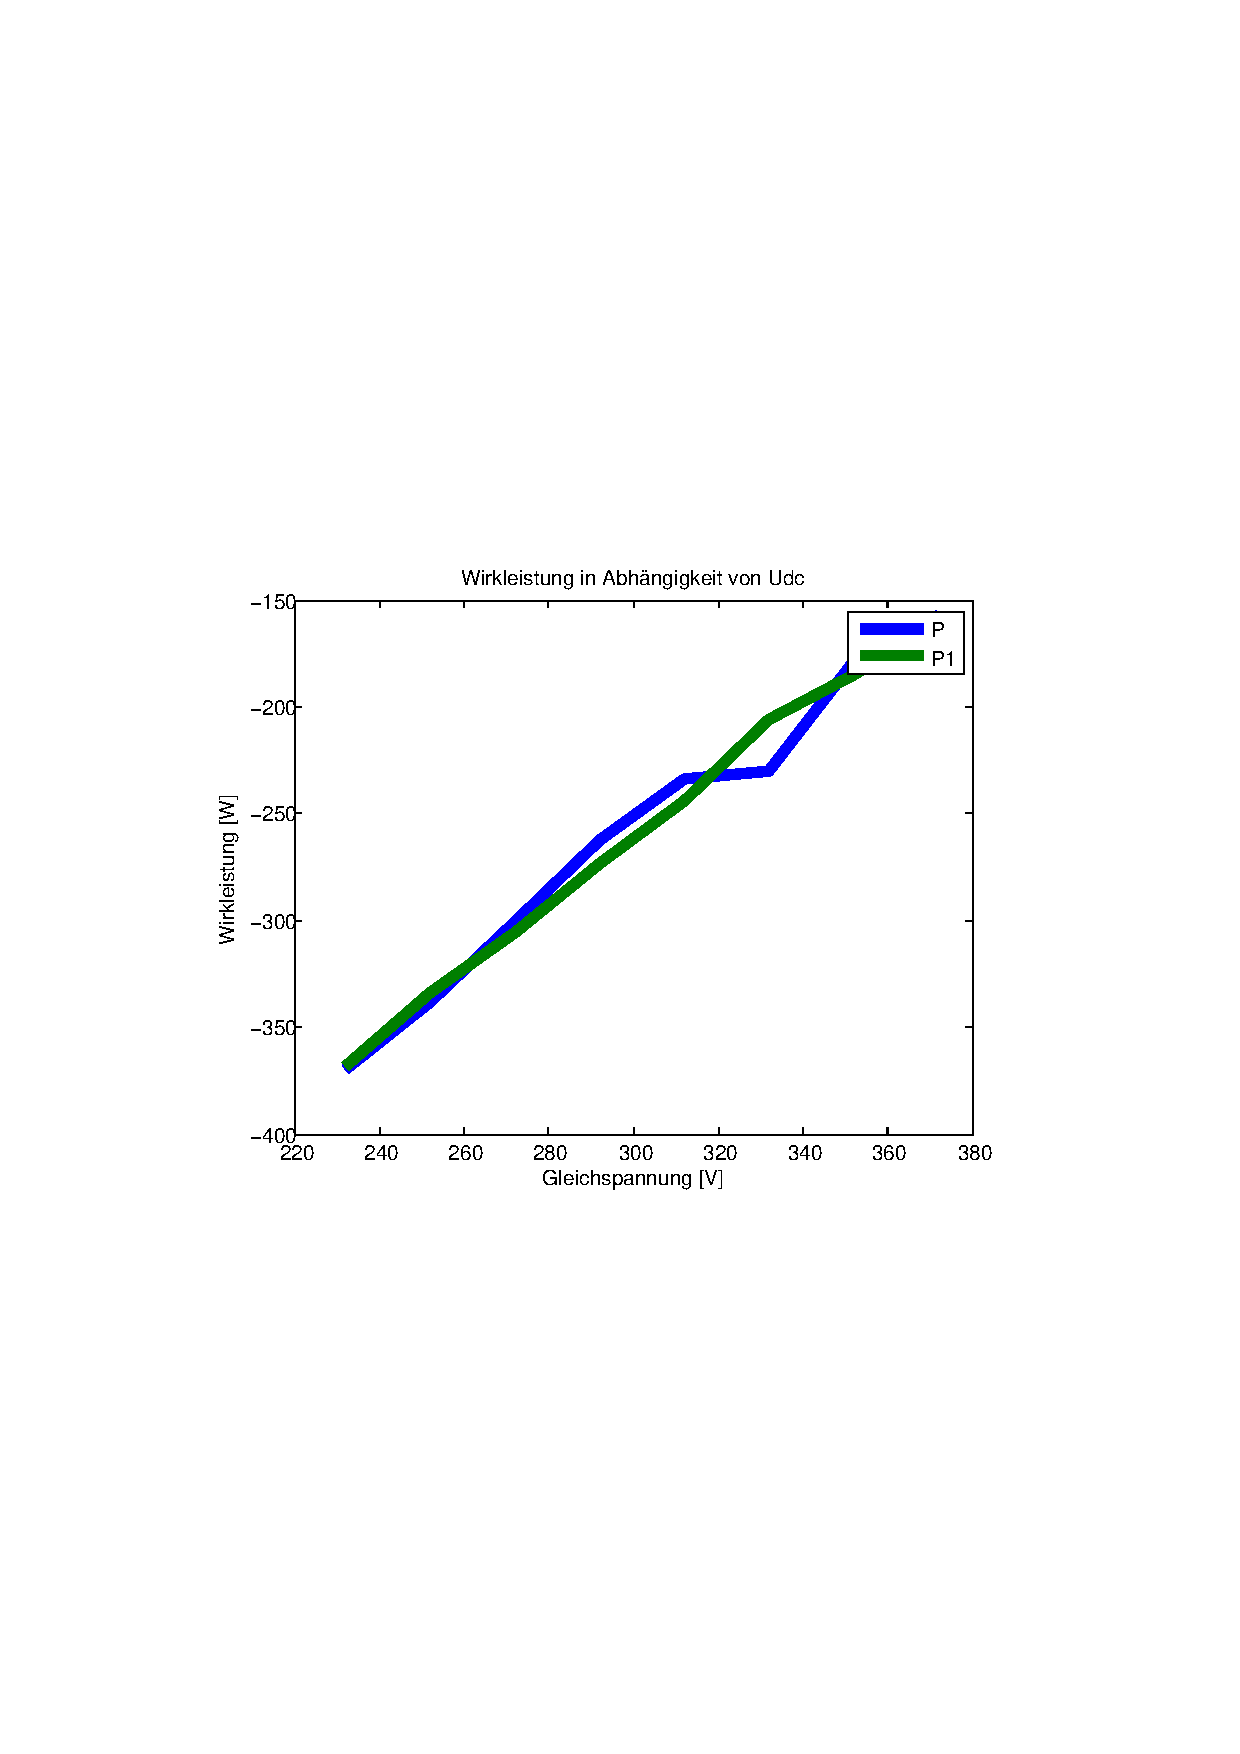
\includegraphics[width=0.5\textwidth, trim={1cm 6.5cm 2cm 7cm},clip]{pic/6_1_grundfrequenztaktung/6_1_2_einst_wirk_und_blindleistung/P_P1_Udc.pdf}
  \caption{Blindleistung $P(U_{DC}) (blau), P1(U_{DC}) (grün)$ in Abhängigkeit der Gleichspannung}
  \label{fig:6_1_2_4}
  \end{center}
\end{figure}


\begin{figure}[H]
  \begin{center}
  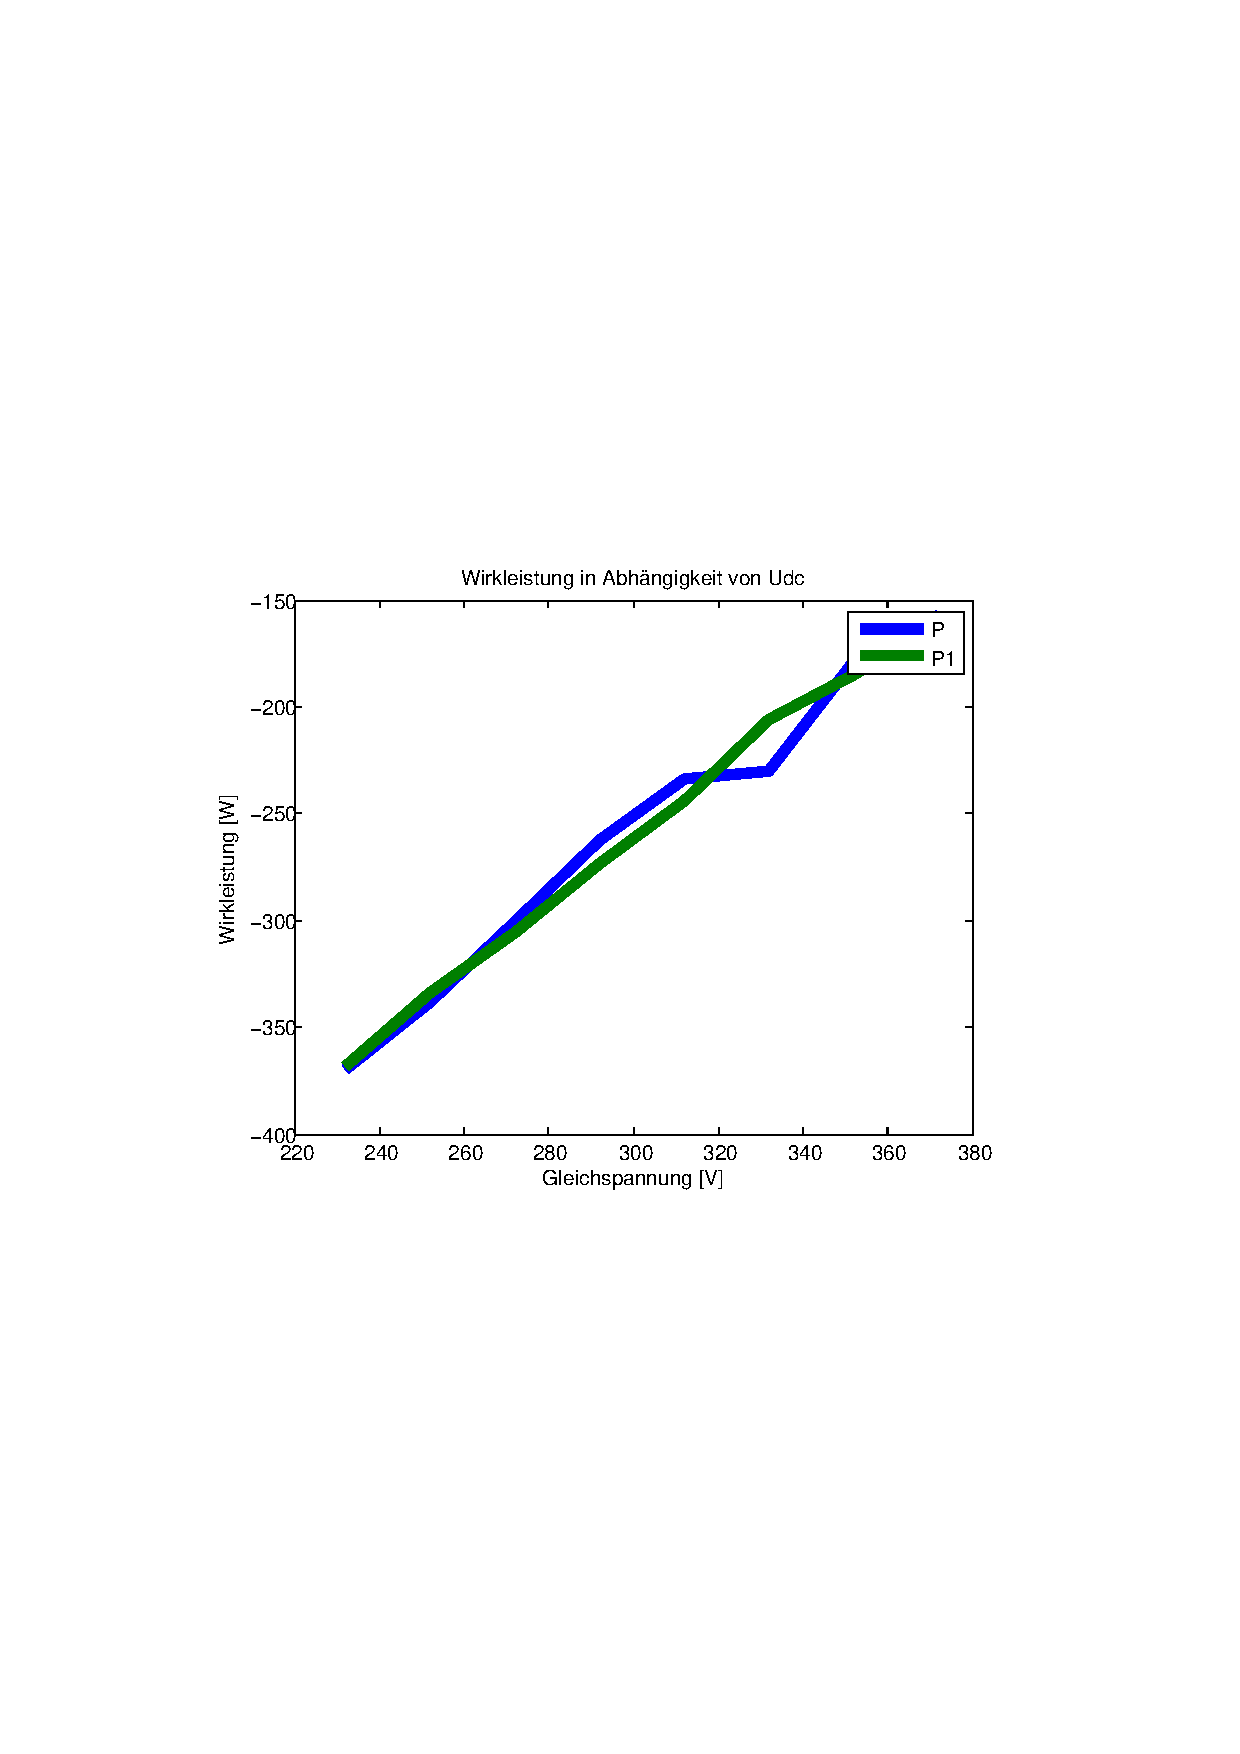
\includegraphics[width=0.5\textwidth, trim={1cm 6.5cm 2cm 7cm},clip]{pic/6_1_grundfrequenztaktung/6_1_2_einst_wirk_und_blindleistung/P_P1_Udc.pdf}
  \caption{Blindleistung $Q(U_{DC}) (blau), Q1(U_{DC}) (grün)$ in Abhängigkeit der Gleichspannung}
  \label{fig:6_1_2_5}
  \end{center}
\end{figure}

\clearpage

\subsection{Weitere Pulsmuster}

\clearpage
\subsubsection{Eliminierung 3 bis 5 Harmonischer}


\begin{figure}[!ht]
  \begin{center}
  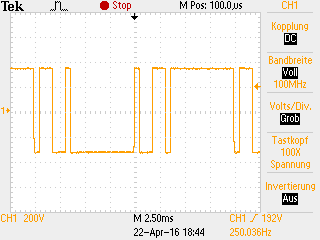
\includegraphics[width=0.48\textwidth]
  {pic/6_2_weitere_pulsmuster/6_2_1_stromform/eliminierung_3_bis_5/ALL0000/F0000TEK.png}
  \caption{$U_A (Orange)$}
  \label{fig:6_2_1_0}
  \end{center}
\end{figure}


\begin{figure}[!ht]
  \begin{center}
  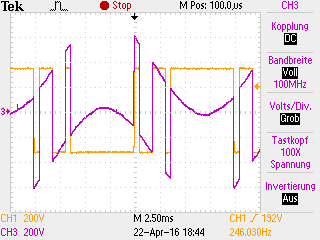
\includegraphics[width=0.48\textwidth]
  {pic/6_2_weitere_pulsmuster/6_2_1_stromform/eliminierung_3_bis_5/ALL0001/F0001TEK.png}
  \caption{$U_A (Orange), U_L (Violett)$}
  \label{fig:6_2_1_1}
  \end{center}
\end{figure}


\begin{figure}[!ht]
  \begin{center}
  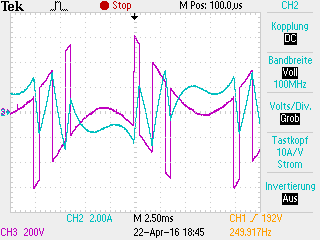
\includegraphics[width=0.48\textwidth]
  {pic/6_2_weitere_pulsmuster/6_2_1_stromform/eliminierung_3_bis_5/ALL0002/F0002TEK.png}
  \caption{$U_L (Violett), I_{L1} (Hellblau)$}
  \label{fig:6_2_1_2}
  \end{center}
\end{figure}


\clearpage
\subsubsection{Eliminierung 3 bis 9 Harmonischer}
Dieses Pulsmuster basiert auf dem selben Prinzip wie jenes im Kapitel \ref{6_2_title}. Jedoch werden hier die [3, 5, 7, 9] Harmonische eliminiert. Um vier Harmonische zu eliminieren, benötigt man vier Freiheitsgrade [$\alpha_1, \alpha_2, \alpha_3, \alpha_4$].\\
\\

Das Ansteuerungssignal hat nun mehrere High-Low-Übergänge, da es nun vier Freiheitsgrade besitzt.
\begin{figure}[H]
  \begin{center}
  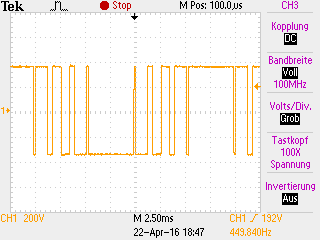
\includegraphics[width=0.48\textwidth]
  {pic/6_2_weitere_pulsmuster/6_2_1_stromform/eliminierung_3_bis_9/ALL0000/F0000TEK.png}
  \caption{$U_A (Orange)$}
  \label{fig:6_2_2_0}
  \end{center}
\end{figure}


\begin{figure}[H]
  \begin{center}
  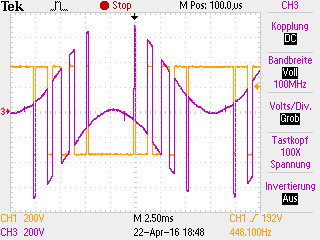
\includegraphics[width=0.48\textwidth]
  {pic/6_2_weitere_pulsmuster/6_2_1_stromform/eliminierung_3_bis_9/ALL0001/F0001TEK.png}
  \caption{$U_A (Orange), U_L (Violett)$}
  \label{fig:6_2_2_1}
  \end{center}
\end{figure}


\begin{figure}[H]
  \begin{center}
  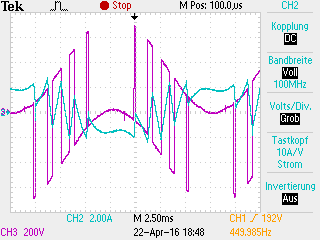
\includegraphics[width=0.48\textwidth]
  {pic/6_2_weitere_pulsmuster/6_2_1_stromform/eliminierung_3_bis_9/ALL0002/F0002TEK.png}
  \caption{$U_L (Violett), I_{L1} (Hellblau)$}
  \label{fig:6_2_2_2}
  \end{center}
\end{figure}

In dem Stromverlauf $I_{L1}$  ist bereits eine Sinusform erkennbar.


\subsubsection{Eliminierung 3 bis 21 Harmonischer}


\begin{figure}[H]
  \begin{center}
  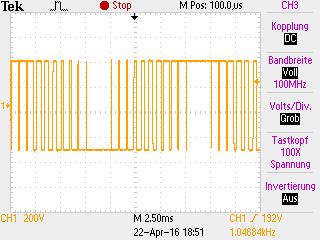
\includegraphics[width=0.48\textwidth]
  {pic/6_2_weitere_pulsmuster/6_2_1_stromform/eliminierung_3_bis_21/ALL0000/F0000TEK.png}
  \caption{$U_A (Orange)$}
  \label{fig:6_2_3_0}
  \end{center}
\end{figure}


\begin{figure}[H]
  \begin{center}
  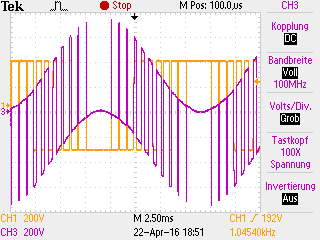
\includegraphics[width=0.48\textwidth]
  {pic/6_2_weitere_pulsmuster/6_2_1_stromform/eliminierung_3_bis_21/ALL0001/F0001TEK.png}
  \caption{$U_A (Orange), U_L (Violett)$}
  \label{fig:6_2_3_1}
  \end{center}
\end{figure}


\begin{figure}[H]
  \begin{center}
  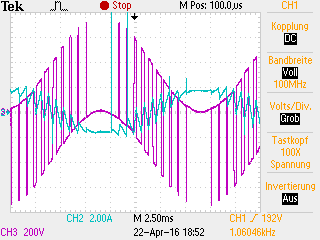
\includegraphics[width=0.48\textwidth]
  {pic/6_2_weitere_pulsmuster/6_2_1_stromform/eliminierung_3_bis_21/ALL0002/F0002TEK.png}
  \caption{$U_L (Violett), I_{L1} (Hellblau)$}
  \label{fig:6_2_3_2}
  \end{center}
\end{figure}


\clearpage
\subsubsection{Sinusträger, grobe Auflösung}


\begin{figure}[H]
  \begin{center}
  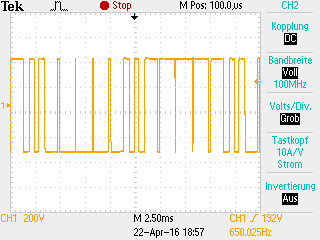
\includegraphics[width=0.48\textwidth]
  {pic/6_2_weitere_pulsmuster/6_2_1_stromform/carrier_grob/ALL0000/F0000TEK.png}
  \caption{$U_A (Orange)$}
  \label{fig:6_2_4_0}
  \end{center}
\end{figure}


\begin{figure}[H]
  \begin{center}
  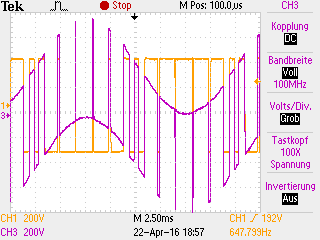
\includegraphics[width=0.48\textwidth]
  {pic/6_2_weitere_pulsmuster/6_2_1_stromform/carrier_grob/ALL0001/F0001TEK.png}
  \caption{$U_A (Orange), U_L (Violett)$}
  \label{fig:6_2_4_1}
  \end{center}
\end{figure}


\begin{figure}[H]
  \begin{center}
  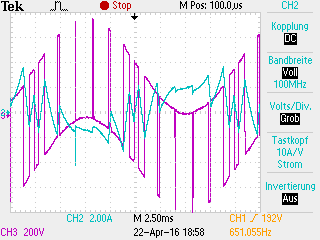
\includegraphics[width=0.48\textwidth]
  {pic/6_2_weitere_pulsmuster/6_2_1_stromform/carrier_grob/ALL0002/F0002TEK.png}
  \caption{$U_L (Violett), I_{L1} (Hellblau)$}
  \label{fig:6_2_4_2}
  \end{center}
\end{figure}


\clearpage
\subsubsection{Sinusträger, feine Auflösung}


\begin{figure}[H]
  \begin{center}
  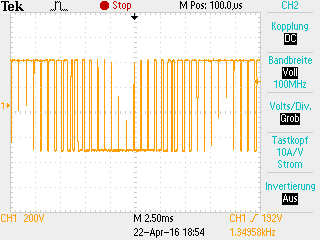
\includegraphics[width=0.48\textwidth]
  {pic/6_2_weitere_pulsmuster/6_2_1_stromform/carrier_fein/ALL0000/F0000TEK.png}
  \caption{$U_A (Orange)$}
  \label{fig:6_2_5_0}
  \end{center}
\end{figure}


\begin{figure}[H]
  \begin{center}
  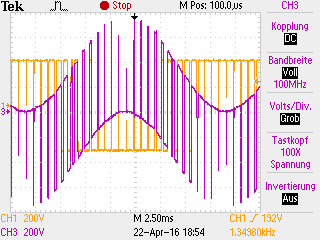
\includegraphics[width=0.48\textwidth]
  {pic/6_2_weitere_pulsmuster/6_2_1_stromform/carrier_fein/ALL0001/F0001TEK.png}
  \caption{$U_A (Orange), U_L (Violett)$}
  \label{fig:6_2_5_1}
  \end{center}
\end{figure}


\begin{figure}[H]
  \begin{center}
  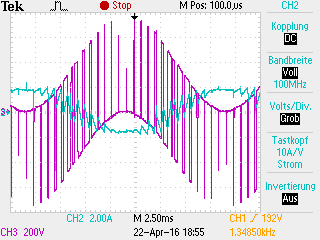
\includegraphics[width=0.48\textwidth]
  {pic/6_2_weitere_pulsmuster/6_2_1_stromform/carrier_fein/ALL0002/F0002TEK.png}
  \caption{$U_L (Violett), I_{L1} (Hellblau)$}
  \label{fig:6_2_5_2}
  \end{center}
\end{figure}



\textbf{Wirk und Blindleistung}\\

\begin{figure}[H]
  \begin{center}
  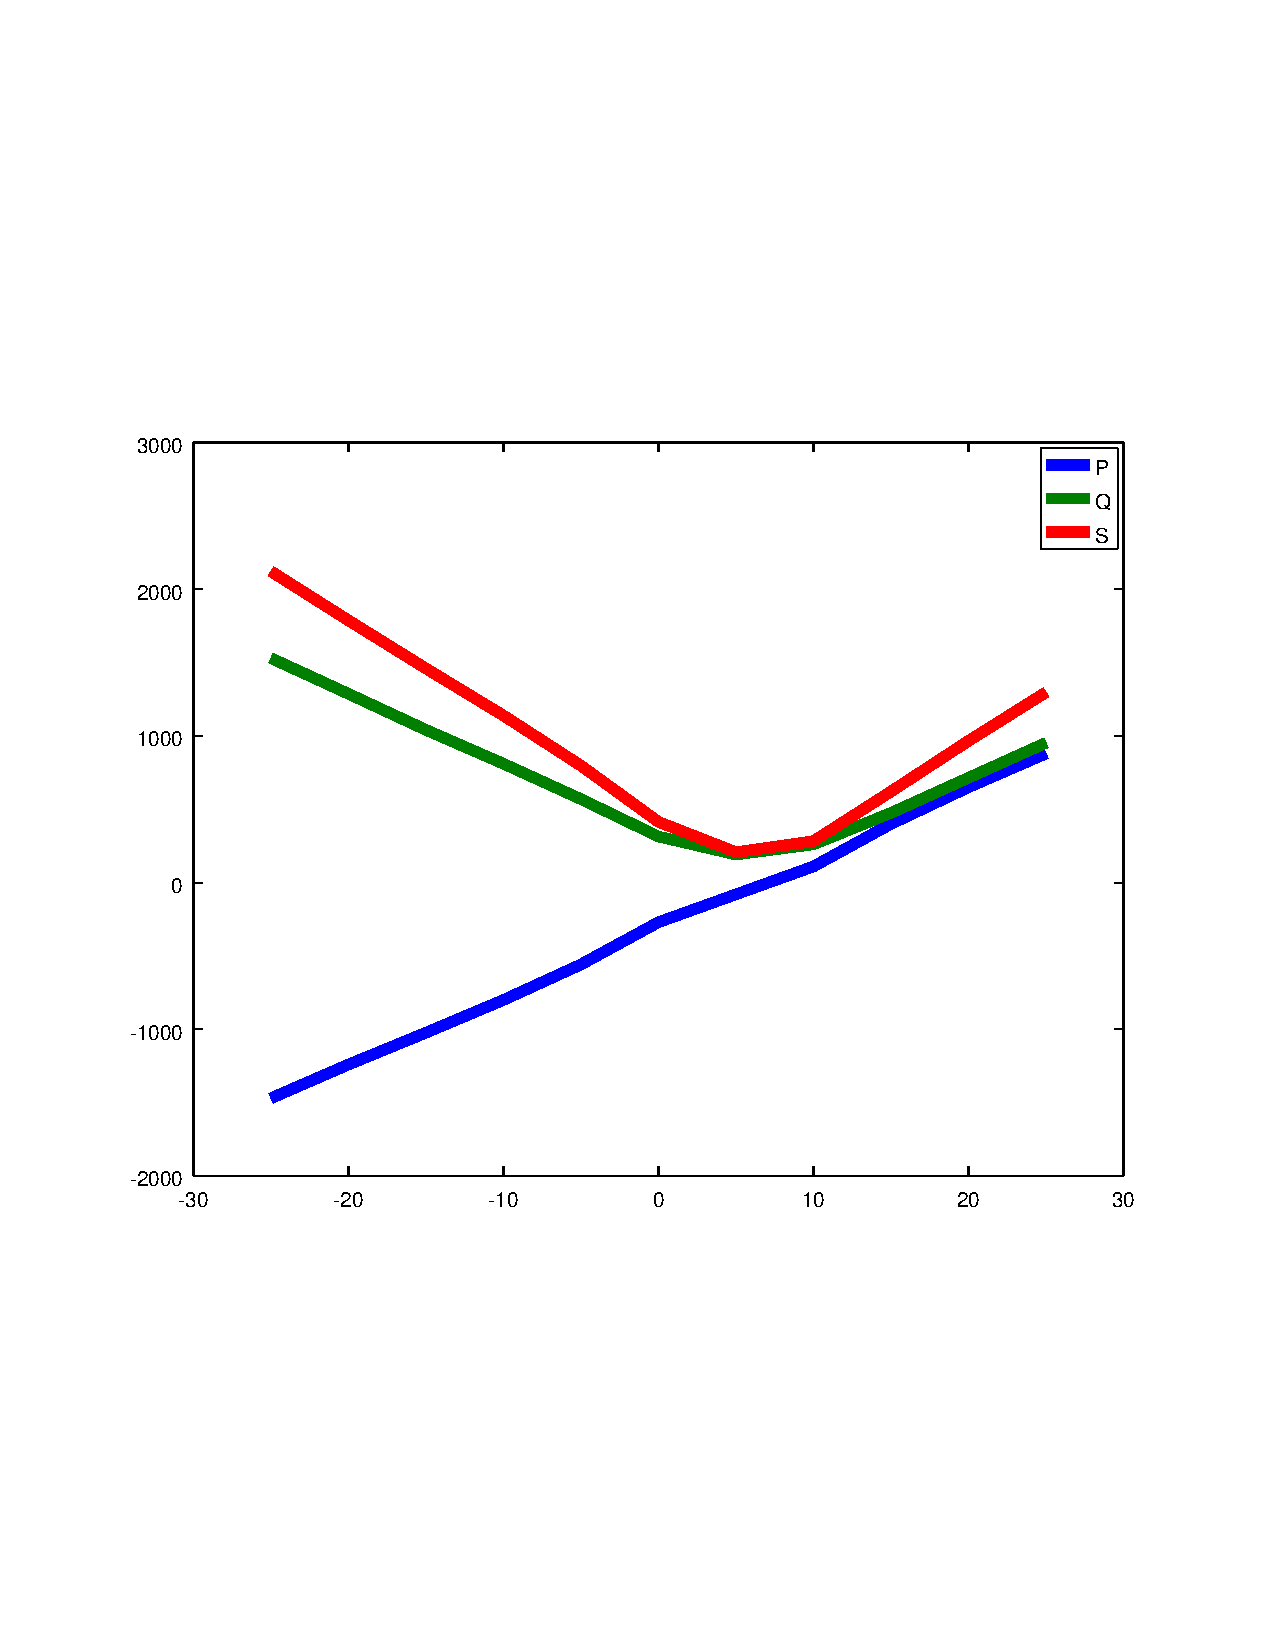
\includegraphics[width=0.5\textwidth, trim={1cm 6.5cm 2cm 7cm},clip]{pic/6_2_weitere_pulsmuster/6_2_2_einst_wirk_und_blindleistung/Sinus_fein_6_2_2_alpha.pdf}
  \caption{$P(\theta), Q(\theta), S(\theta)$}
  \label{fig:6_1_5_3}
  \end{center}
\end{figure}


\begin{figure}[H]
  \begin{center}
  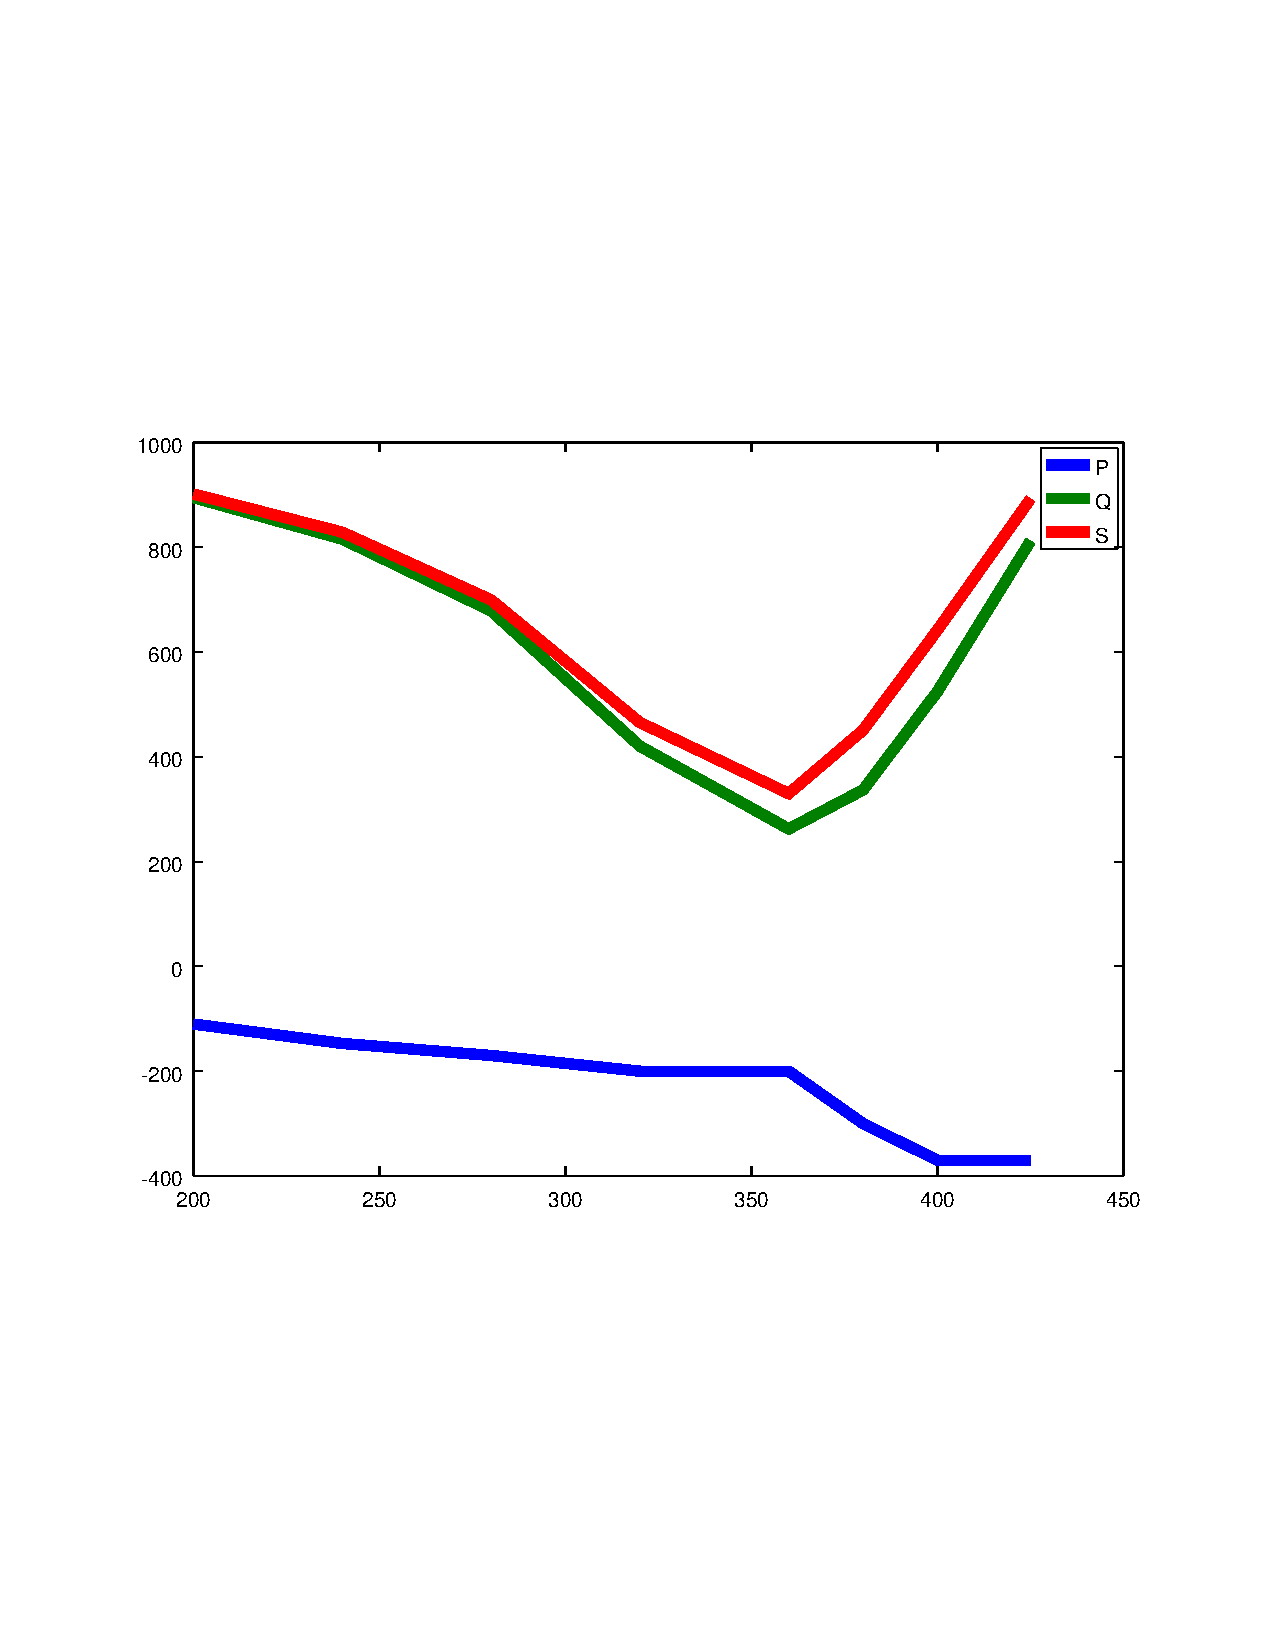
\includegraphics[width=0.5\textwidth, trim={1cm 6.5cm 2cm 7cm},clip]{pic/6_2_weitere_pulsmuster/6_2_2_einst_wirk_und_blindleistung/Sinus_fein_6_2_2_udc.pdf}
  \caption{$P(U_{dc}), Q(U_{dc}), S(U_{dc})$}
  \label{fig:6_1_5_4}
  \end{center}
\end{figure}

\clearpage



%\subsection{Spannungsbelastung der Halbleiter}

\clearpage
%\subsection{Diverse Messungen}

\clearpage



% Messgeräte
\section{Messgeräte}

\begin{tabular}{ l | l | l }
  \hline 
  Inv. Nummer & Name & Verwendung \\
  \hline \hline
  545 & Tektronix TPS2014 & Strom-, Spannungs-Messung  \\
  \hline
  120 & PM3000 A & Strom-, Spannungs-Messung für die harmonischen  \\  
  \hline
  
  xxx & DA 1000VN, Differentialmesssonde  \\  
  \hline
  xxx & DA 1000VN, Differentialmesssonde  \\  
  \hline
  
  xxx & PR 30 & Stromzange  \\  
  \hline
  xxx & PR 30 A & Stromzange  \\  
  \hline
  
\end{tabular}



\noindent




%Anhang
\clearpage
\section{Anhang}
\appendix
\section{Aufgabenstellung}

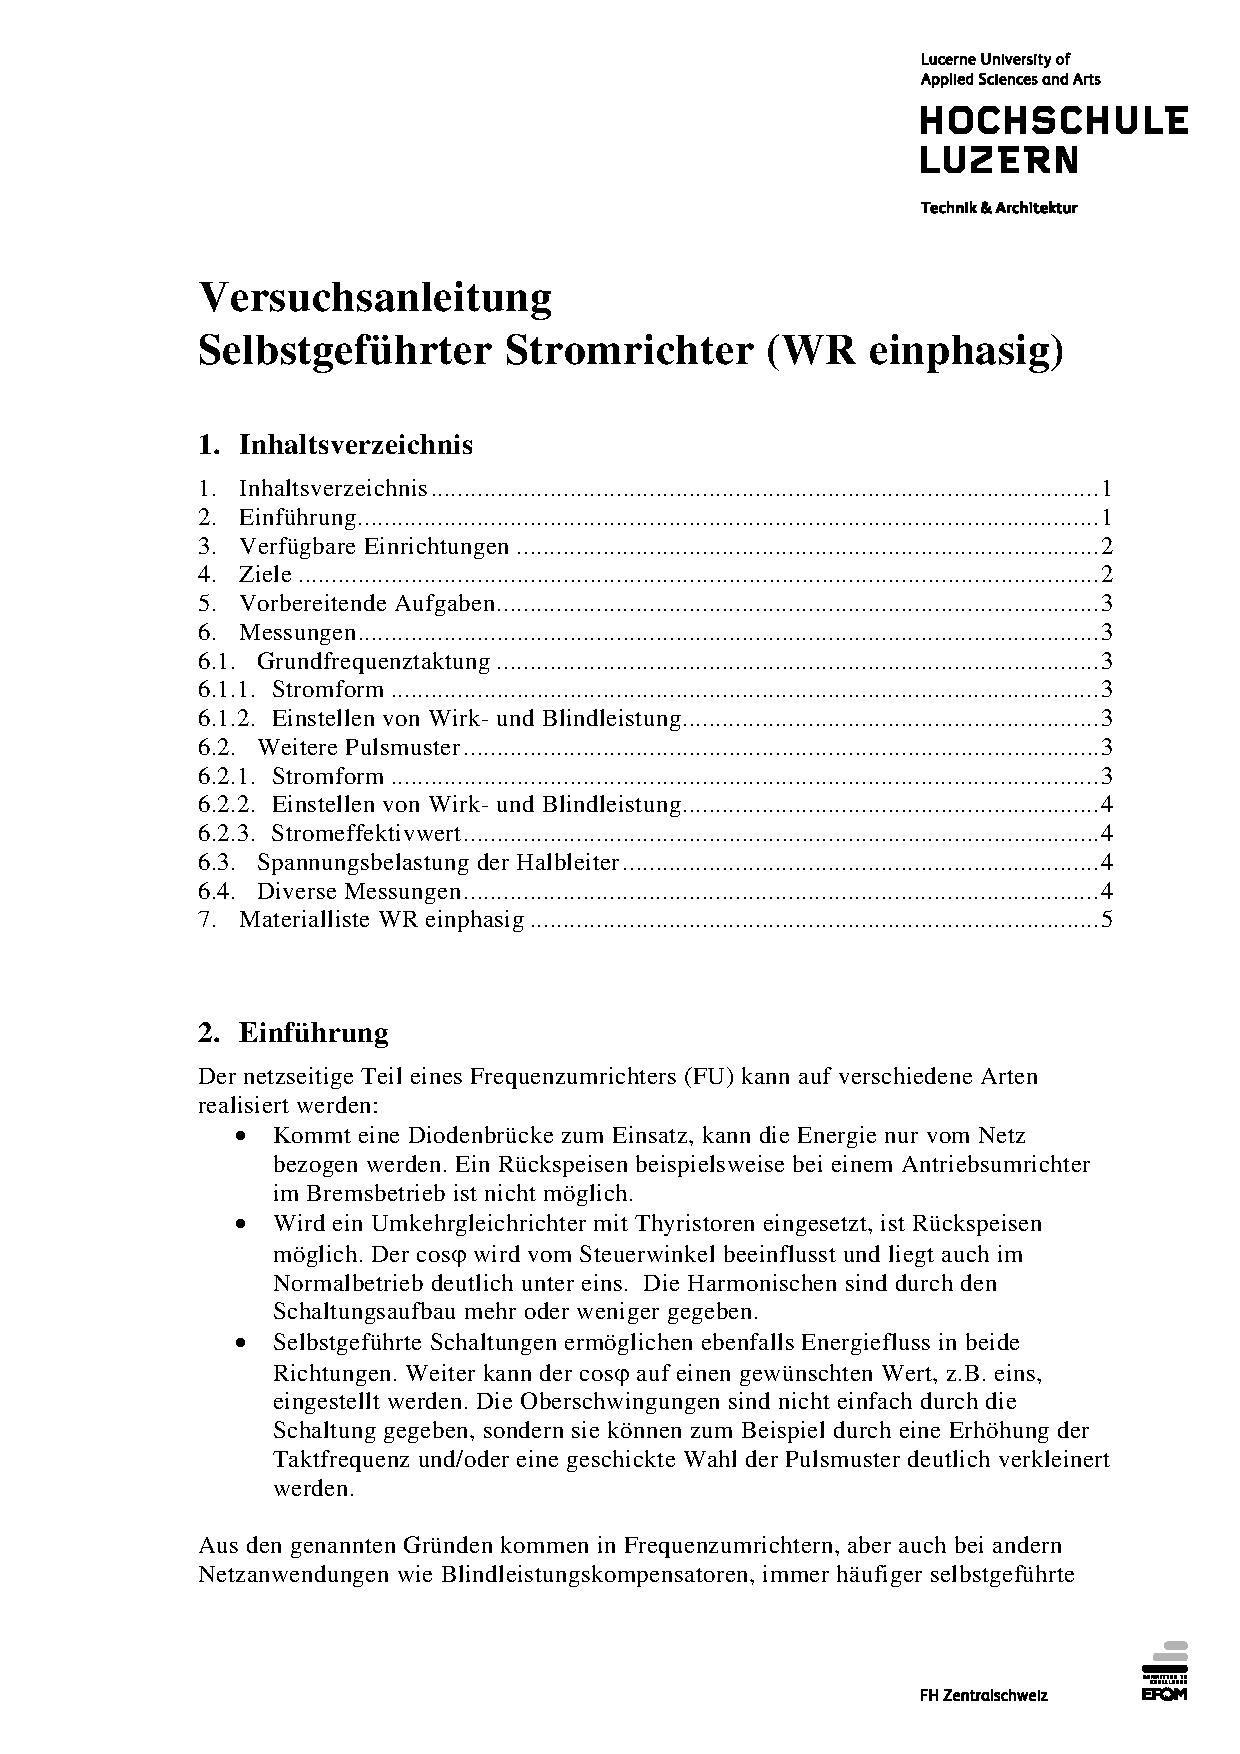
\includepdf[pages={-}]{pic/99_appendix/Laboranleitung_WR_einphasig.pdf}




\end{document}